\documentclass[14pt]{report}
\usepackage{geometry}                % See geometry.pdf to learn the layout options. There are lots.
\geometry{letterpaper}                   % ... or a4paper or a5paper or ... 
%\geometry{landscape}                % Activate for for rotated page geometry
%\usepackage[parfill]{parskip}    % Activate to begin paragraphs with an empty line rather than an indent
\usepackage{graphicx}
\usepackage{amssymb}
\usepackage{epstopdf}
\DeclareGraphicsRule{.tif}{png}{.png}{`convert #1 `dirname #1`/`basename #1 .tif`.png}

\begin{document}
\section{Bayesian regression}
\begin{figure}[h!]
  \caption{The variance of the posterior at k=1 against N }
  \centering
    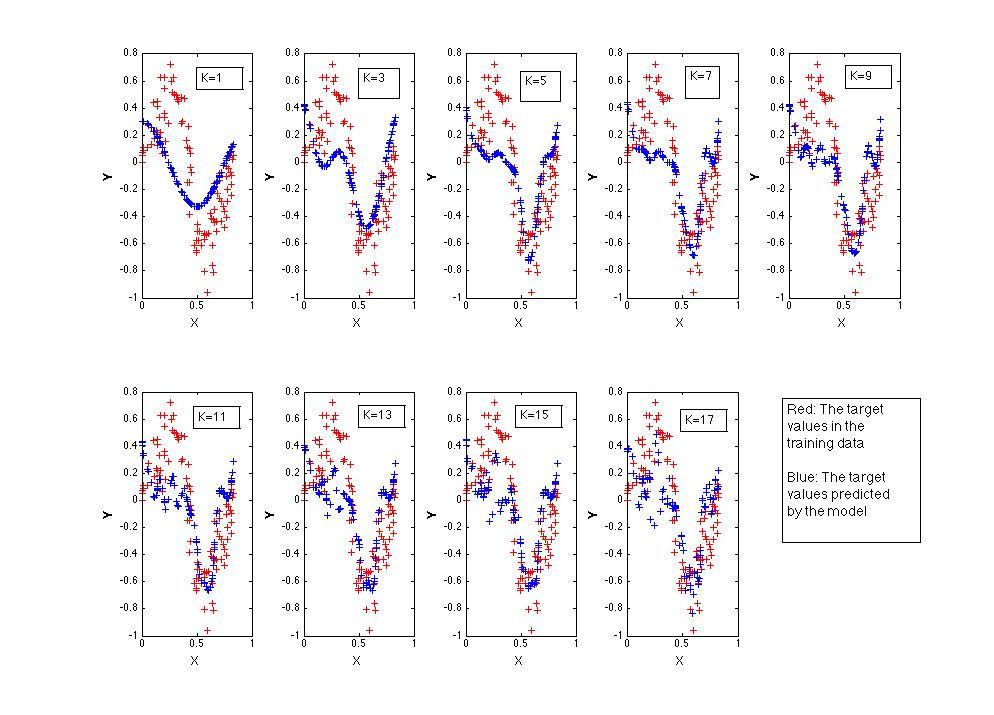
\includegraphics[width=0.8\textwidth]{4A.jpg}
\end{figure}
\begin{figure}[h!]
  \caption{The variance of the posterior at k=1 against N }
  \centering
    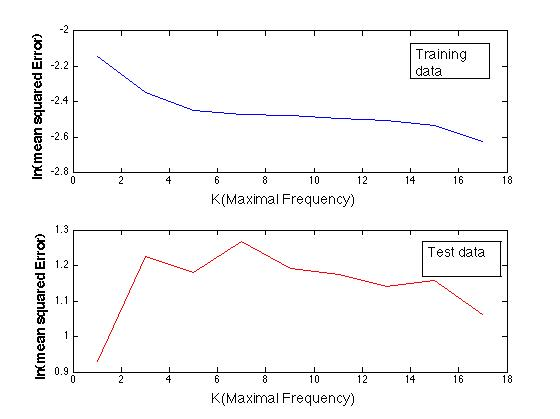
\includegraphics[width=0.8\textwidth]{4b.jpg}
\end{figure}
\begin{figure}[h!]
  \caption{The variance of the posterior at k=1 against N }
  \centering
    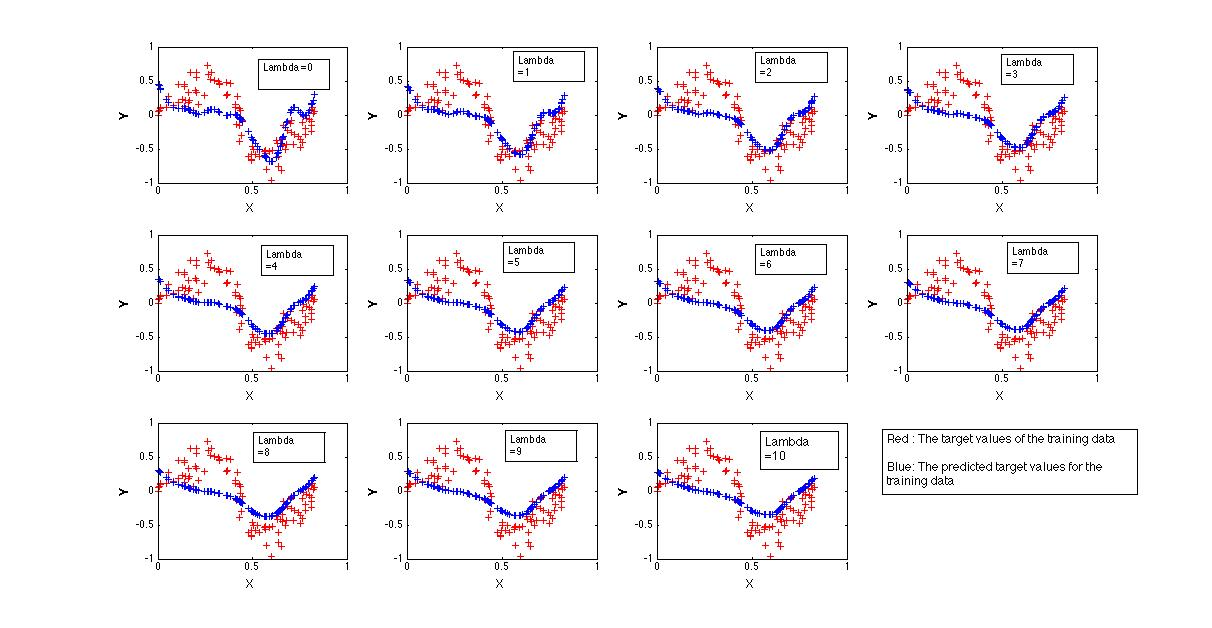
\includegraphics[width=0.8\textwidth]{4C.jpg}
\end{figure}
%\section{}
%\subsection{}



\end{document}  